\section*{Problem 3: Portfolio Choice}
\begin{enumerate}
\item
FOC with respect to $\alpha$, we can have 
$$E\left[\left(1+r^{f}+\alpha(r-r^{f})\right)^{-\gamma_{i}}(r-r^{f})\right]$$
the solution of the equation is the optimal portfolio share for each agent $i$.
\item

If we use the parametrization of problem 2, which is $r^{f}=0.02$, $r^{\text{min}}=-0.08$ and $r^{\text{max}}=0.12$ with the probability of 0.5, respectively, then the problem can be written as 
\begin{align*}
0.5\times\left[(1.02+0.1\alpha)^{-\gamma_{i}}\times0.1\right]&+0.5\times\left[(1.02+(-0.1)\alpha)^{-\gamma_{i}}\times0.1\right]=0\\
\Leftrightarrow ~~(1.02+0.1\alpha)^{-\gamma_{i}}&=(1.02-0.1\alpha)^{-\gamma_{i}}
\end{align*}
Then it will lead to $\alpha=0$, regardless of $\gamma_{i}$.

When I set $p=0.8$, the plot of $\alpha$ against $\gamma_{i}$ looks as follows,
\begin{figure}[htbp]
\centering
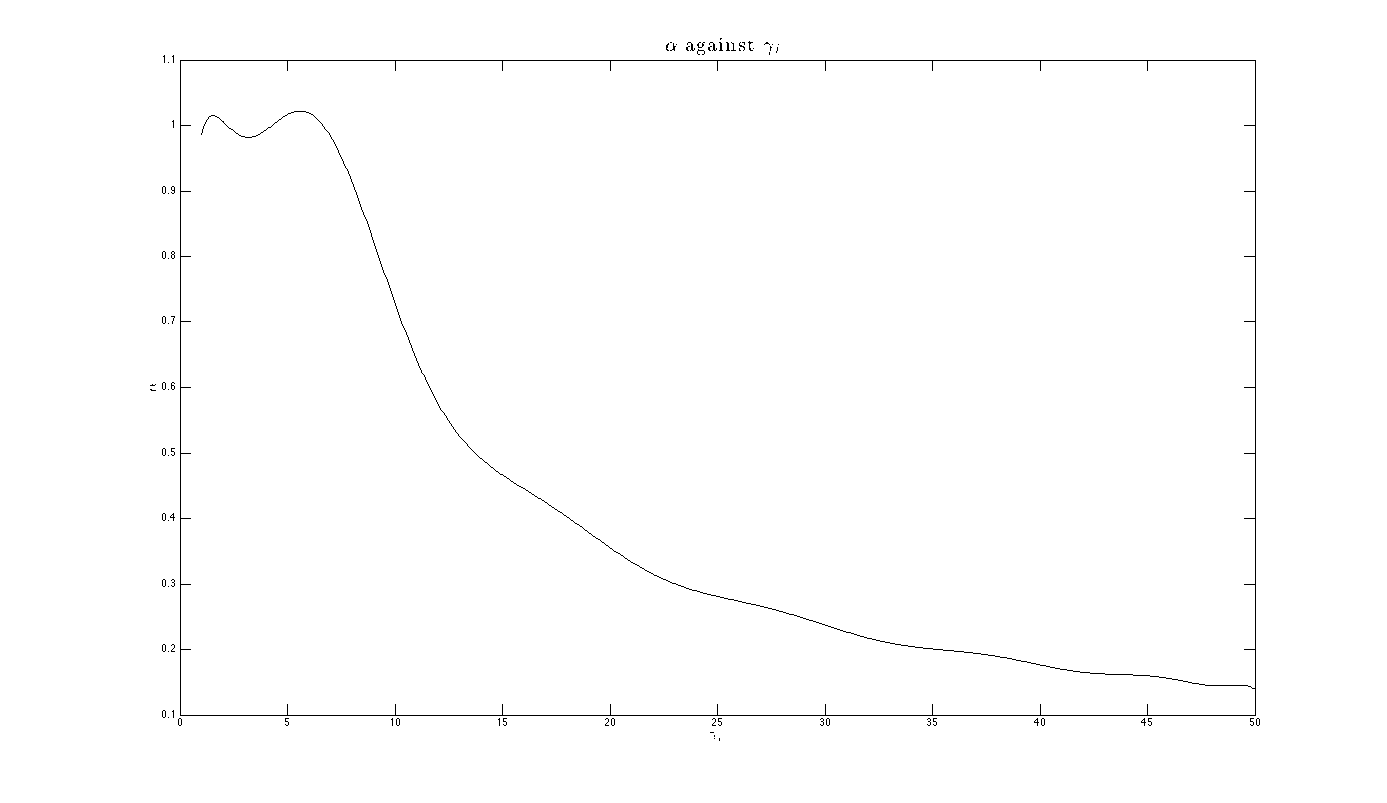
\includegraphics[width=\linewidth]{Figure/Q3.png}
\end{figure}
From the figure, we can observe that in the neighborhood of the point where $\alpha$ is binding, the points are not exactly smooth at 1 due to the characteristics of the basic function.

\item
\begin{figure}[htbp]
\centering
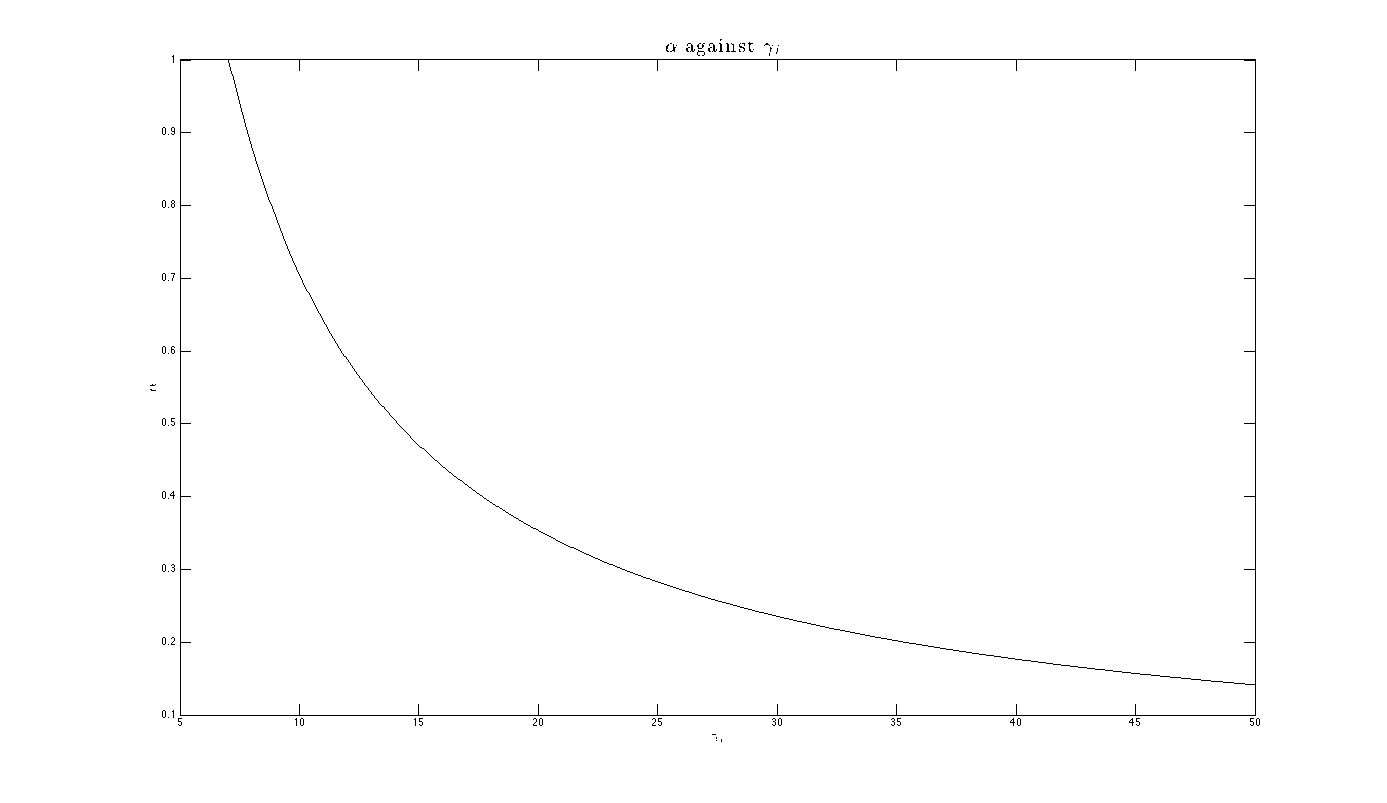
\includegraphics[width=\linewidth]{Figure/Q3_2.png}
\end{figure}
$\bar{\gamma}=7.04$ when $\alpha$ is just binding.\\
The graph now looks smoother than before.
\end{enumerate}